\section{Multi-name models of default}
We consider credit derivatives whose underlying is a set of names (reference entities). A multi-name contract is associated with multiple credit events which trigger remedial payment to the protection buyer. The collateralized debt obligation (CDO) is one of the most popular multi-name credit derivatives. We want to look at the default correlation.

\subsection{A structual approach}
To model the default correlation consider the Black-Scholes-Merton (BSM) structural model of default with default defined as

$$
\tau= \begin{cases}T, & \text { if } V_{T}<F \\ \infty & \text { if } V_{T} \geq F\end{cases}
$$

where $F$ is the face value of the debt and $V_{T}$ is the asset values at maturity. Hence, it is the asset values $V_{T}$ at maturity $T$ that is the quantity of interest. Assuming $T=1$ and defining the return on the asset values $\tilde{R}$ over the period from 0 to $T$ as

$$
\mathrm{e}^{\tilde{R}}=\frac{V_{1}}{V_{0}}=\frac{V_{0} \mathrm{e}^{\left(\mu-\frac{\sigma^{2}}{2}\right)}}{V_{0}}
$$

where the last equality holds since $V_{T}$ is log-normally distributed in the BSM model. Taking the logarithm on both sides we have

$$
\tilde{R} \sim N\left(\mu-\frac{\sigma^{2}}{2}, \sigma^{2}\right)
$$

Likewise, the default can be written in terms of the return on the asset value

$$
\begin{gathered}
V_{1}<F, \\
\widehat{\Downarrow} \\
\tilde{R}=\ln \left(\frac{V_{1}}{V_{0}}\right)<\ln \left(\frac{F}{V_{0}}\right), \\
\widehat{\Downarrow} \\
R=\frac{\tilde{R}-\left(\mu-\frac{\sigma^{2}}{2}\right)}{\sigma}<\frac{\ln \left(\frac{F}{V_{0}}\right)-\left(\mu-\frac{\sigma^{2}}{2}\right)}{\sigma}=C,
\end{gathered}
$$

where $R$ is the standardized return on the firm value and the right hand side is a constant $C$. Thus, default of the firm can be written as

$$
R<C
$$

where $R$ is standard normally distributed.

\section{Introducing several companies}
We define the default of company $i$ as when the standardized return on owning the firm falls below a firm specific threshold $C_{i}$ at some future time $T$

$$
\text { Company } i \text { defaults at time } T \Longleftrightarrow R_{i} \leq C_{i}, \quad R_{i}=\frac{\tilde{R}_{i}-\mathbb{E}\left[\tilde{R}_{i}\right]}{\sqrt{\mathbb{V}\left[\tilde{R}_{i}\right]}}
$$

The standardization means all $R_{i}$ s in the portfolio have zero mean and unit variance. We assume that individual period returns $R_{i}$ are normally distributed. Thus, the default probabilities are

$$
q_{i}=\mathbb{Q}\left[R_{i} \leq C_{i}\right]=\Phi\left(C_{i}\right) \quad \Longrightarrow \quad C_{i}=\Phi^{-1}\left(q_{i}\right)
$$

with $\Phi(\cdot)$ the CDF of the standard normal distribution. Furthermore, assume that all returns are correlated through one common factor $\alpha$ by

$$
R_{i}=\beta_{i} \alpha+\sqrt{1-\beta_{i}^{2}} \epsilon_{i}
$$

where $\alpha$ and $\epsilon_{i}$ are independent and standard normally distributed. Also, the $\epsilon_{i}$ s are independent. (The common factor $\alpha$ could be interpreted as the standardized return on the stock market or the general state of the economy).

How are company returns correlated in this setting?

$$
\begin{aligned}
\operatorname{Cov}\left(R_{i}, R_{j}\right) & =\mathbb{E}\left[\left(R_{i}-\mathbb{E}\left[R_{i}\right]\right)\left(R_{j}-\mathbb{E}\left[R_{j}\right]\right)\right] \\
& =\mathbb{E}\left[R_{i} R_{j}\right] \\
& =\mathbb{E}\left[\beta_{i} \beta_{j} \alpha^{2}\right] \\
& =\beta_{i} \beta_{j} \\
& =\operatorname{corr}\left(R_{i}, R_{j}\right),
\end{aligned}
$$

since all the other random variables involved are independent and we have unit variance. Key advantage: Given a common factor $\alpha$ the returns are independent, observed by

$$
\begin{aligned}
& \mathbb{E}\left[R_{i} \mid \alpha\right]=\beta_{i} \alpha \\
& \mathbb{V}\left[R_{i} \mid \alpha\right]=\mathbb{E}\left[\left(R_{i}-\beta_{i} \alpha\right)^{2} \mid \alpha\right]=\mathbb{E}\left[\left(1-\beta_{i}^{2}\right) \epsilon_{i}^{2} \mid \alpha\right]=1-\beta_{i}^{2}
\end{aligned}
$$

Now, we can find the correlation of the returns given knowledge of the common factor $\alpha$

$$
\operatorname{Cov}\left(R_{i}, R_{j} \mid \alpha\right)=\sqrt{1-\beta_{i}^{2}} \sqrt{1-\beta_{j}^{2}} \mathbb{E}\left[\epsilon_{i} \epsilon_{j} \mid \alpha\right]=0
$$

since individual factors were assumed independent. From this, the convenient form of the default probability given $\alpha$ arises

$$
\begin{aligned}
q_{i}(\alpha) & =\mathbb{Q}\left[R_{i} \leq C_{i} \mid \alpha\right] \\
& =\mathbb{Q}\left[\left.\epsilon_{i} \leq \frac{C_{i}-\beta_{i} \alpha}{\sqrt{1-\beta_{i}^{2}}} \right\rvert\, \alpha\right] \\
& =\Phi\left(\frac{C_{i}-\beta_{i} \alpha}{\sqrt{1-\beta_{i}^{2}}}\right) \\
& =\Phi\left(\frac{\Phi^{-1}\left(q_{i}\right)-\beta_{i} \alpha}{\sqrt{1-\beta_{i}^{2}}}\right)
\end{aligned}
$$

which depends on $\beta_{i}$.

What are the correlation of defaults $\rho_{i, j}$ ? It has the form form

$$
\rho_{i, j}=\frac{q_{i \& j}-q_{i} q_{j}}{\sqrt{q_{i}\left(1-q_{i}\right)} \sqrt{q_{j}\left(1-q_{j}\right)}}=\frac{\Phi_{2}\left(C_{i}, C_{j} ; \beta_{i} \beta_{j}\right)-\Phi\left(C_{i}\right) \Phi\left(C_{j}\right)}{\sqrt{\Phi\left(C_{i}\right)\left(1-\Phi\left(C_{i}\right)\right)} \sqrt{\Phi\left(C_{j}\right)\left(1-\Phi\left(C_{j}\right)\right)}},
$$

using $q_{i}(\alpha)=\Phi\left(C_{i}\right)$ and that $R_{i}$ and $R_{j}$ are bivariate normally distributed with correlation coefficient $\operatorname{corr}\left(R_{i}, R_{j}\right)=\beta_{i} \beta_{j}$ so

$$
q_{i \& j}=\mathbb{Q}\left[R_{i} \leq C_{i} \text { and } R_{j} \leq C_{j}\right]=\Phi_{2}\left(C_{i}, C_{j} ; \beta_{i} \beta_{j}\right)
$$

\subsection{Additional stuff}
The loss distribution function: Most multi-name credit derivatives depend on the losses incurred in the portfolio. Hence, the object of interest is the loss distribution function that assigns probabilities to default related losses over some time horizon. Assuming $\beta_{i}=\beta, C_{i}=C$ and $R_{i}=R$ the loss $L$ relates to the number of defaults $k$ by

$$
L=\frac{k}{I}(1-R)
$$

where $I$ is the number of entities. The number of defaults on a portfolio is binomially distributed (individual returns $R_{i}$ were independent given $\alpha$ ) given $\alpha$, so the individual conditional default probability is

$$
q(\alpha)=\Phi\left(\frac{C-\beta \alpha}{\sqrt{1-\beta^{2}}}\right)
$$

Large portfolio approximation: When the number of entities $I$ in the portfolio is high, the CDF for the losses gets numerically hard to work with. Instead we can use the large portfolio approximation

$$
\mathbb{Q}[L \leq \theta]=\Phi\left(-\frac{\Phi^{-1}(q)-\Phi^{-1}(\theta) \sqrt{1-\beta^{2}}}{\beta}\right)
$$

CDOs: Two types:

\begin{itemize}
  \item Traditional: CDO is based on the payoffs from an underlying pool of loans/bonds.
  \item Synthetic: CDO is a "pure" credit derivative, which again can be build from traditional CDOs.\\
The basic principle in both is to split the payments associated with an underlying pool of assets into different tranches with different seniority. Buyer gets money from seller in case of defaults.\\
Pricing CDO tranches: $K_{L_{j}}$ and $K_{U_{j}}$ are attachment and detachment point of tranche $j . Z_{j, t}$ is the loss percentage incurred on tranche $j$ at time $t$
\end{itemize}

$$
Z_{j, t}=\min \left\{Z_{t}, K_{U_{j}}\right\}-\min \left\{Z_{t}, K_{L_{j}}\right\}
$$

The spread on tranche $j$ is

$$
s_{j}=\frac{\sum_{k=1}^{K} B_{0}^{T}\left(\mathbb{E}\left[Z_{j, t_{k}}\right]-\mathbb{E}\left[Z_{j, t_{k-1}}\right]\right)}{\sum_{k=1}^{K} B_{0}^{T} \eta\left(K_{U_{j}}-K_{L_{j}}-\mathbb{E}\left[Z_{j, t_{k}}\right]\right)},
$$

\begin{figure}[H]
\begin{center}
  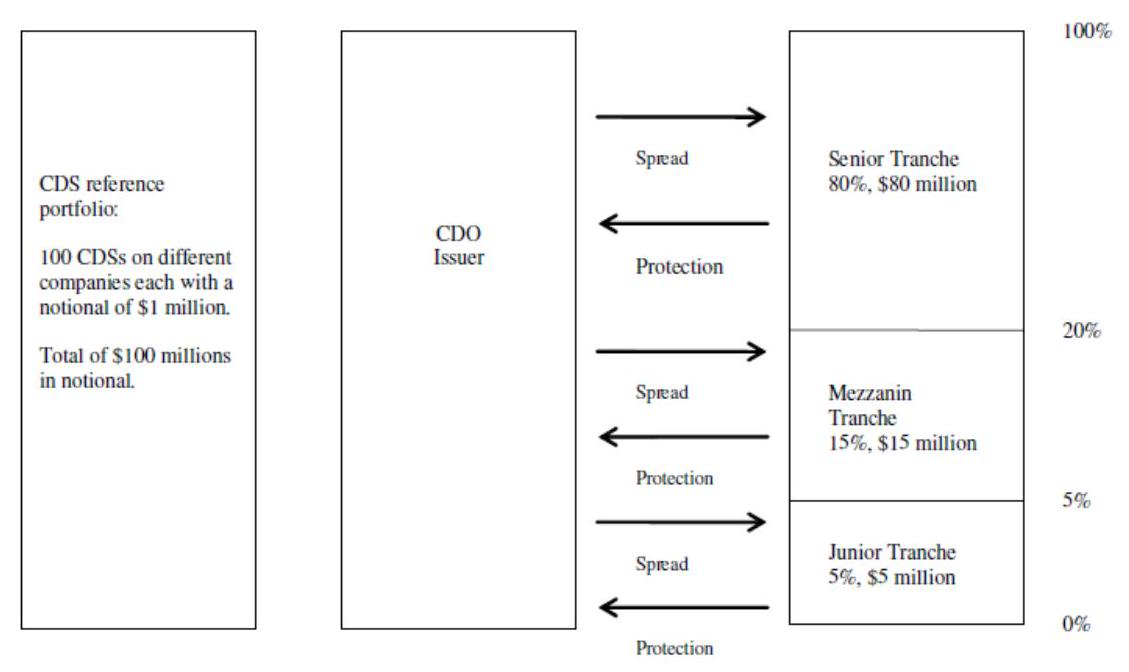
\includegraphics[width=0.8\textwidth]{figures/cdo.jpg}
\captionsetup{labelformat=empty}
\caption{Figure: Structure in an unfunded synthetic CDO.}
\end{center}
\end{figure}

with $\eta$ being grid size. Using LPA, pricing of a tranche boils down to evaluating

$$
\mathbb{E}\left[Z_{j, t_{k}}\right]=\int_{0}^{1} \min \left\{(1-R) \theta, K_{U_{j}}\right\}-\min \left\{(1-R) \theta, K_{L_{j}}\right\} \mathrm{d} F\left(\theta ; q_{t_{k}}, \beta\right)
$$

where

$$
F\left(\theta ; q_{t_{k}}, \beta\right)=\Phi\left(-\frac{\Phi^{-1}\left(q_{t_{k}}\right)-\Phi^{-1}(\theta) \sqrt{1-\beta^{2}}}{\beta}\right) .
$$

\section{Fixed income issues after 2008 (CVA, pricing collateralized claims)}
Idea: Let's model explicitly the credit risk and the liquidity risk in the interbank market and measure/calibrate our model.

Swap contracts are collateralized and therefore swap rates have negligible counterparty risk component. Thus, variation in swap contracts comes only from variation in the floating reference rate. The difference between a 5 year swap on LIBOR (rates for unsecured lending and borrowing between banks) and the 5 year swap on OIS (risk free interest rate proxy, rate at which banks can borrow from each other over night) comes from the difference between (risk neutral) expectations between LIBOR and OIS rates over the next 5 years. The difference between swap rates on contracts referencing different LIBOR rates are mainly due to liquidity risk (i.e. a premium is required for lending out money for longer horizons). LIBOR-OIS spread - measure of risk in the interbank market.

\subsection{Pricing collateralized claims}
Consider a contract with payoff/cashflow $X$ and maturity $T . V(t, T)$ is the present value of $X$. Posting of cash-collateral on a continuous marking-to-market basis ( $100 \%$ of $V(t, T)$, best practice among financial institutions is daily). The receiver of the collateral can invest it at the risk-free rate $r(t)$ and has to pay an agreed rate $r_{c}(t)$ to the poster of the collateral

$$
V(t)=\mathbb{E}_{t}^{\mathbb{Q}}\left[\mathrm{e}^{-\int_{t}^{T} r(u) \mathrm{d} u} X+\int_{t}^{T} \mathrm{e}^{-\int_{t}^{u} r(s) \mathrm{d} s}\left(r(u)-r_{c}(u)\right) V(u) \mathrm{d} u\right]
$$

To valuate the payoffs we discount

$$
\mathrm{e}^{-\int_{0}^{t} r(u) \mathrm{d} u} V(t)=\mathbb{E}_{t}^{\mathbb{Q}}\left[\mathrm{e}^{-\int_{0}^{T} r(u) \mathrm{d} u} X+\int_{t}^{T} \mathrm{e}^{-\int_{0}^{u} r(s) \mathrm{d} s}\left(r(u)-r_{c}(u)\right) V(u) \mathrm{d} u\right]
$$

We denote

$$
M(t)=\mathrm{e}^{-\int_{0}^{t} r(u) \mathrm{d} u} V(t)+\int_{0}^{t} \mathrm{e}^{-\int_{0}^{u} r(s) \mathrm{d} s}\left(r(u)-r_{c}(u)\right) V(u) \mathrm{d} u
$$

which is a $\mathbb{Q}$-martingale (all discounted price processes are MG under $\mathbb{Q}$ ), so

$$
\mathrm{d}\left(\mathrm{e}^{-\int_{0}^{t} r(u) \mathrm{d} u} V(t)\right)=-\left(r(t)-r_{c}(t)\right)\left(\mathrm{e}^{-\int_{0}^{t} r(u) \mathrm{d} u} V(t)\right) \mathrm{d} t+\mathrm{d} M(t)
$$

With integrations by parts we obtain

$$
\begin{aligned}
\mathrm{d}\left(\mathrm{e}^{-\int_{0}^{t} r_{c}(u) \mathrm{d} u} V(t)\right)= & \mathrm{d}\left(\mathrm{e}^{\int_{0}^{t} r(u)-r_{c}(u) \mathrm{d} u} \mathrm{e}^{-\int_{0}^{t} r(u) \mathrm{d} u} V(t)\right) \\
= & \left(r(t)-r_{c}(t)\right) \mathrm{e}^{\int_{0}^{t} r(u)-r_{c}(u) \mathrm{d} u}\left(\mathrm{e}^{-\int_{0}^{t} r(u) \mathrm{d} u} V(t)\right) \mathrm{d} t \\
& +\mathrm{e}^{\int_{0}^{t} r(u)-r_{c}(u) \mathrm{d} u}\left(-\left(r(t)-r_{c}(t)\right) \mathrm{e}^{-\int_{0}^{t} r(u) \mathrm{d} u} V(t) \mathrm{d} t+\mathrm{d} M(t)\right) \\
= & \mathrm{e}^{\int_{0}^{t} r(u)-r_{c}(u) \mathrm{d} u} \mathrm{~d} M(t)
\end{aligned}
$$

Since $\mathrm{e}^{-\int_{0}^{t} r_{c}(u) \mathrm{d} u} V(t)$ is a $\mathbb{Q}$-martingale and $V(T)=X$ we have

$$
\mathrm{e}^{-\int_{0}^{t} r_{c}(u) \mathrm{d} u} V(t)=\mathbb{E}_{t}^{\mathrm{Q}}\left[\mathrm{e}^{-\int_{0}^{T} r_{c}(u) \mathrm{d} u} X\right]
$$

and conclude that the payoffs can be computed by

$$
V(t)=\mathbb{E}_{t}^{\mathbb{Q}}\left[\mathrm{e}^{-\int_{t}^{T} r_{c}(u) \mathrm{d} u} X\right]
$$

\subsection{Credit valuation adjustment}
Considering bilateral counterparty risk is essential in the post-crisis landscape as risky counterparties otherwise would not be able to agree upon a price. Incorporating bilateral counterparty features in a model can explain seemingly paradoxical statements. If the counterparty in a contract defaults, the market value of the contract can be lost for the outher counterpaty. In case the contract is a CDS it only makes sense to use a model that allows for a stochastic future market value (e.g. by stochastic default intensity).

CVA - "How much do I discount the price of this deal due to the fact that my counterparty can default?" (the default risk of my counterparty). Assume your own default probability is zero. Then the CVA is defined as the difference between the value of the contract assuming the counterparty is risk-free and the actual value of the contract

$$
\begin{aligned}
\text { Value of claim } & =\text { Default-free value of claim }- \text { CVA } \\
\pi & =\pi^{\text {Default-free }}+\text { CVA }
\end{aligned}
$$

The CVA is most difficult to value when the contract has payments in both directions between the two counterparties (e.g. interest rate swap or credit default swap). An additional layer of complexity is added as we are hurt by a counterparty default when the contract has positive value for us, but not when is has negative value.

Defining the exposure at time $t$ as

$$
X_{t}^{+}=\max \left\{\epsilon_{t}, 0\right\}
$$

where $\epsilon_{t}$ is the close-out amount (the amount of the losses or costs the surviving party would incur in replacing or in providing for an economic equivalent of the remaining part of the deal at the time when the counterparty defaults). The pricing formula for CVA is then

$$
\mathrm{CVA}_{t}=-\mathbb{E}_{t}^{\mathrm{Q}}\left[\mathrm{e}^{-\int_{t}^{\tau} r_{s} \mathrm{~d} s}\left(1-R_{E C_{2}}\right) X_{\tau}^{+} \mathbb{1}_{\left\{\tau=\tau_{2} \leq T\right\}}\right]
$$

\section{Additional stuff}
\subsection{Mean reversion}
Ornstein-Uhlenbeck process: $\mathrm{d} x_{t}=\kappa\left(\theta-x_{t}\right) \mathrm{d} t+\beta \mathrm{d} z_{t}$. The process is mean reverting towards $\theta$ (the mean). $\kappa$ decides "how fast" it returns. $\beta$ is the degree of volatility. If $x_{t}$ is above $\theta, \kappa$ is multiplied by a negative number and the variable goes down, and vice versa.

\begin{figure}[H]
\centering
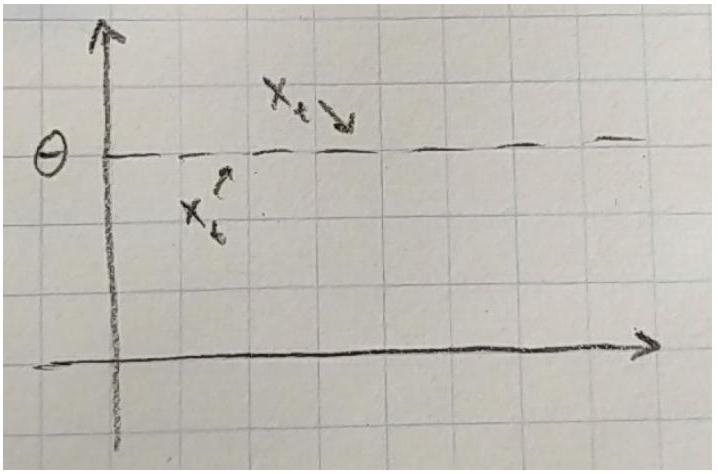
\includegraphics[width=0.8\textwidth]{figures/mean-reversion.jpg}
\end{figure}




\subsection{Credit risk}
Definition: The risk that an obligor does not honor his payments due to a default event.\\
Credit risky products are of interest to banks (and other financial institutions) because credit derivatives gives them the possibility to trade credit risk and export it out of the balance sheet. With credit derivatives it is possible to hedge the credit risk of their own portfolios.

For investors it is interesting to trade in corporate bonds and credit derivatives since the decreasing interest rate level has made corporate bonds and the higher yield on these more interesting compared to government bonds. With credit derivatives it is possible to tailor-make the credit portfolio to match the investors risk profile.

\begin{itemize}
  \item Credit Default Swap: Suppose a bank (protection buyer) enters into a contract with an investment firm (protection seller), where it will make periodic payments to the firm in exchange for a lump sump if XYC corp. (refenrence entity) defaults during the contract term. The lump sum is denoted ( $1-R$ ) (assuming notional 1) and the CDS spread is determined so the contract has value zero at initiation.
  \item Collaterized Debt: Multi-name instrument. A collection of portfolio default swaps.
  \item Portfolio default swap: The protection seller covers losses in the portfolio between the attachment point and the detachment point in exchange for a periodic payment. The contract is terminated at the maturity of the contract or until the total loss in the portfolio exceeds the detachment point.
  \item First to default basket: A basket of reference names. The protection seller agrees to cover the loss of the first default in the basket in return for a periodic payment.\\
Valuation principles: The valuation at time zero corresponds to: protection leg $=$ premium leg.
\end{itemize}

